\chapter{Grundlagen}

In diesem Kapitel werden alle verwendeten Komponenten und Technologien kurz erläutert.

\section{LR-WPAN - IEEE 802.15.4}

LR-WPAN steht für \grqq Low Rate - Wireless personal area network \grqq{}. Es handelt sich also um eine Kabelloses geschlossenes Netzwerk, welches für 
niedrige Datenraten ausgelegt ist. Der Standard definiert den Physical Layer sowie den Media-Access Layer und ist Grundlage von ZigBee, Thread, 6LowPAN.
Im Standard sind mehrere Modulationsverfahren sowie Frequenzbereiche definiert. Peer-to-Peer ist Teil des Standards. Der Medium-Access Layer baut nicht
auf 802.1d, es handelt sich also nicht um klassische MAC-Pakete. Die Adressen sind kürzer und die Pakete kleiner. 

\section{ZigBee}

Die ZigBee Alliance wurde durch ein Konsortium von Herstellern gegründet, um einen einheitlichen Übertragungstandard
im Bereich Heimautomatisierung voranzubringen. ZigBee basiert auf einem offenem IEEE Standard, bringt allerdings Komponenten mit die nicht in einem IEEE
Standard definiert sind.
ZigBee ist in Form von weiteren Protokollschichten implementiert, welche auf IEEE 802.15.4 aufsetzen. ZigBee nutzt DSSS, also Frequenzspreizung als Modulationsverfahren
und die Kanäle (11 - 26) liegen im 2,4 Ghz Band. Zigbee interferiert damit mit WLAN.

\begin{figure}[H]
  \centering
  \includegraphics[width=1\textwidth]{media/Zigbee Stack.jpg}
  \caption{ZigBee Protocoll Stack \\ Bildquelle: \url{https://www.researchgate.net/figure/IEEE820154-ZigBee-protocol-stack-architecture_fig2_265150617}}
\end{figure}

Genutzt wird es, um Geräte, wie zum Beispiel Lampen, Schalter oder Thermostate
zur Kommunikation zu befähigen. Dies kann genutzt werden um die Geräte zu steuern, sowie aktuelle Zustandsdaten abzufragen. 
Markante Eigenschaft ist, dass die Geräte keine direkte Funkverbindung
zu einem zentralen Controller brauchen. Einzelne Geräte können als Router fungieren. Dies sorgt dafür,
dass mir einer geringen Sendeleistung ein geografisch großes Gebiet abgedeckt werden kann. Sende- und Empfangsleistung
ist vorallem bei kleinen Batteriebetriebenen Geräten der einschränkende Faktor.


\section{Texas Instruments CC Chips}

Texas Instruments bietet ein Spektrum von Microcontrollern, die sich mit entsprechender Firmware für ZigBee Devices 
nutzen lassen können. Kleinere Chips können in Enddevices wie Lampen, größere als Koordinator selbst verwendet werden.

Die aktuelle Chipfamilie TexasInstruments CC26XX:

\begin{figure}[H]
  \centering
  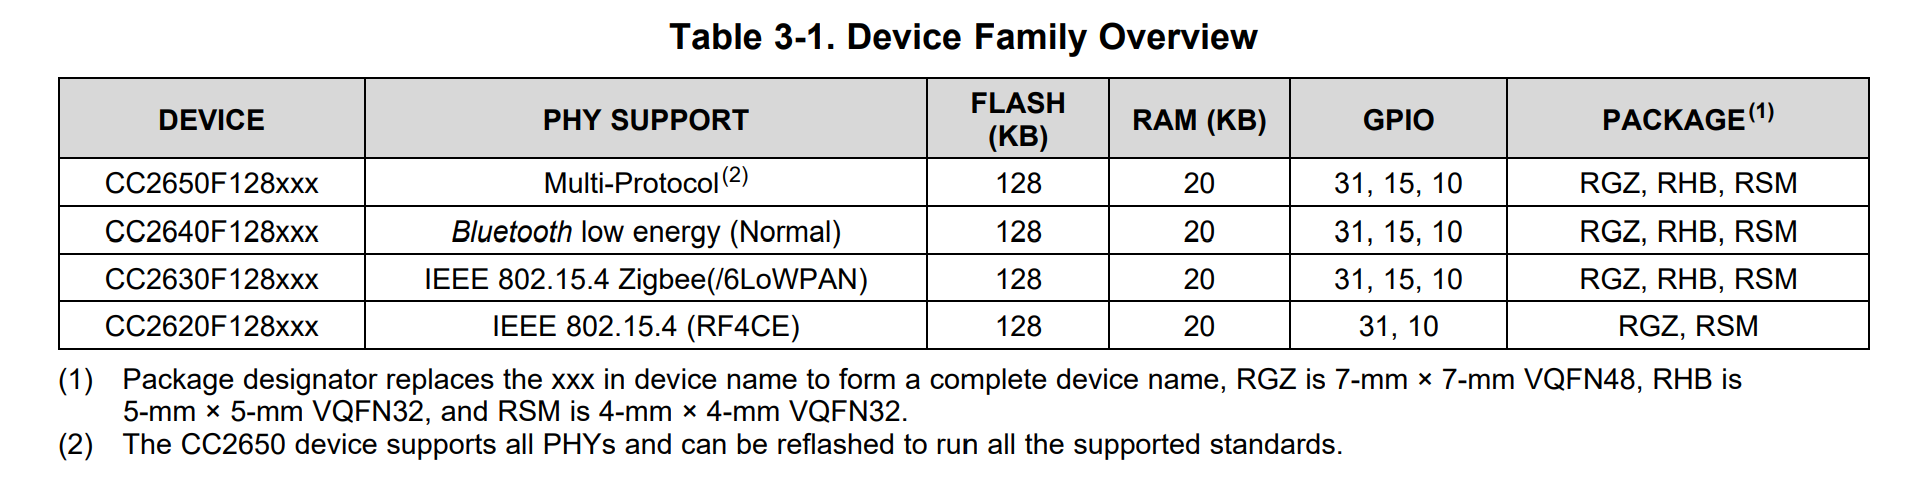
\includegraphics[width=1\textwidth]{media/table26xx.png}
  \caption{Test des Messagebrokers Mosquitto}
\end{figure}

Als Koordinator werden die Leistungsfähigeren Chips aus der 265X Reihe eingesetzt. ZigBee Geräte nutzen in einigen
Fällen Bluetooth LE zur Koppelung, daher ist die Unterstüzung diesen Protokolls sinnvoll.

\begin{figure}[H]
  \centering
  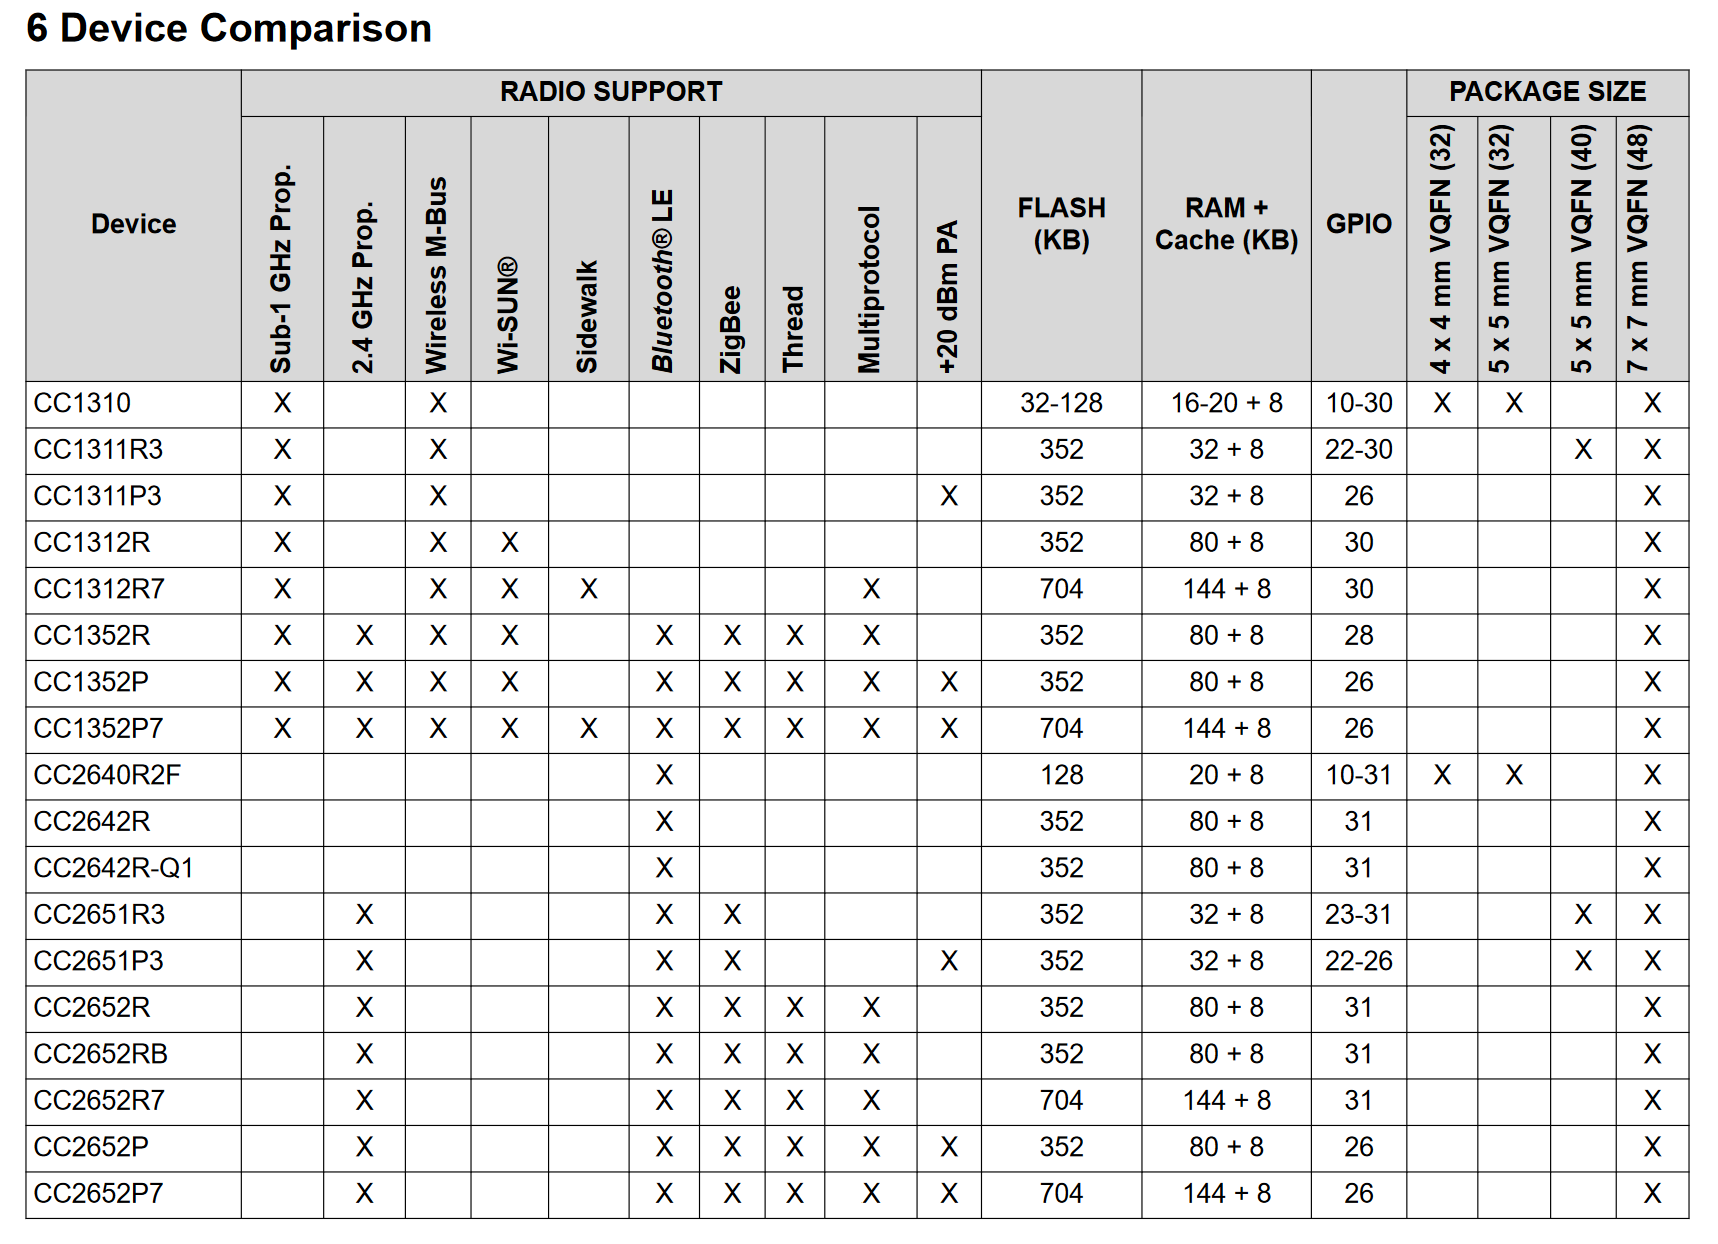
\includegraphics[width=1\textwidth]{media/table265x.png}
  \caption{TI CC 265X Serie}
\end{figure}

In der Tabelle sind die unterstützten Protokolle der einzelnen Modelle sowie deren Leistungsfähigkeit aufgeführt.
Es ist anzumerken, dass die Top Modelle schon den Standard Thread unterstützen, der vermutlich durch das
Projekt \grqq Matter\grqq{} erheblich an bedeutung gewinnt.

Texas Instruments bietet als Basis für ZigBee Eigententwicklungen eine Z-Stack Bibliothek. Diese stellt alle grundlegende 
Funktionen um das ZigBee Protokoll zu implementieren. Mit TexasInstruments Code Composer Studio steht eine IDE bereit,
um den Entwicklungsprozess zu unterstützen. Auf den entsprechend Leistungsfähigeren Chips lassen sich so noch zusätzliche
Funktionalitäten einprogrammieren. Die Chips können mit Programmierboards des Herstellern programmiert werden. Alternativ kann man
günstig einen USB-Stick mit aufgelöteten CC Chip erwerben, und auch diesem mit entsprechenden Tools programmieren.

Weiter Informationen: \url{https://www.ti.com/tool/Z-STACK#overview}

In dem OpenSource Projekt "zigbee2mqtt" werden ausschließlich Chips von Texas Instruments unterstützt. Es sei erwähnt, 
dass die meißten gängigen Anbieter von Microchips entsprechende Modelle im Angebot haben. 

\section{Versuchshardware}

\subsection{RaspberryPi}

Der RaspberryPi ist ein ARM basierter Computer im Mini-Format. Er dient in diesem Versuch als Server, der die Applikationen
hostet und gleichzeitig als Versuchs-PC, auf dem der Versuch durchgeführt wird. Die eingesetzten Anwendungen sind 
als Webservice implementiert.

Der RaspberryPi besitzt die Nutzer PC typtischen Schnittstellen wie Ethernet, HDMI, sowie USB. Als Hauptspeicher wird eine
SD-Karte eingestzt. 

Auf dem RaspberryPi wird das Linux-basierte Betriebssystem RaspbianOS eingesetzt. 

\subsection{RaspberryPi Zigbee Hat}

Als Zigbee Koordinator wird ein auf dem TI CC2652 basierendem RaspberryPi Hat vom Hersteller \grqq cod.m \grqq{} eingesetzt. Dieser wurde vom Hersteller
für den Einsatz mit \grqq homegear \grqq{} oder \grqq zigbee2Mqtt \grqq{} entwickelt. Ein Datenblatt sowie ein Manual ist im Anhang.

\subsection{CC2235 Sniffer Stick}

Mit diesem Stick wird die ZigBee Kommunikation zwischen dein einzelnen Devices sowie dem Koordinator mitgeschnitten.
Der stick basiert auf einem leistungsschwachen Chip, der mit entsprechender Firmware empfangende Pakete empfängt und über die USB Schnittstelle
berfügbar macht. 

\url{https://github.com/virtualabs/cc2531-killerbee-fw}

\subsection{Phillips Hue Komponenten}

Die Phillips Hue Serie setzt vollständig auf den ZigBee Standard auf. Die Produkte haben ein eigenes Öko-System mit entsprechender App und Gateway. Sie sind Kompatibel
zu dem Software-Gateway zigbee2mqtt.
Die Lampen werden in dem Versuch als Demonstrationsobjekte eingesetzt. Sie können Ein- und Ausgeschaltet werden, sowie gedimmt werden. Zusätzlich wird einer
Phillips Hue Fernbedienung verwendet, die zur Steuerung der Lampen dient. Phillips verwendet bei kleinen Geräten die ZigBee Chips von Atmel, bei größeren 
sind auch Eigenentwicklungen zu finden.

\section{Eingesetzte Software}

\subsection{Raspbian OS}

RaspbianOS ist eine leichtgewichtige Linux Distribution, welche direkt vom Hersteller des RaspberryPis speziell auf die Bedürfnisse des Board angepasst werden. Es enthällt eine
Desktop Umgebung sowie die grundlegende Paketen. Es basiert auf Debian, damit sind auch die entsprechenden Paketquellen verfügbar. Durch die große Verbreitung 
sind viele Anwendungen für das Betriebssystem verfügbar.

\subsection{Docker}

Docker ist eine Container Umgebung, um Anwendungen containerisiert auf Linux-Servern ausführen zu können. Docker reduziert erheblich den Aufwand 
Anwendungen zu betreiben. Alle Abhängigkeiten sind im Container enthalten, sodass hier keine Komplikationen mit anderen Anwendungen
zu befürchten sind oder Abhängigkeiten fehlen. Prozesse laufen in eigenen Namespaces und sind dadurch abgekoppelt vom Host Betriebssystem. Im Unterschied zur Virtualisierung werden
Systemprozesse gemeinsam genutzt. Dadurch ist die Effizienz höher als bei taditioneller Virtualisierung.

\subsection{Docker-Compose}

Docker-Compose ist ein Tool, um große Containerumgebungen per YAML zu definieren und automatisch deployen. Klassisch kann ein Container 
per CLI Befehl mit entsprechenden Parametern gestartet werden:
\begin{lstlisting}
  docker run hello-world -v ./home:/home -p 80:80
\end{lstlisting}
Start des Container \grqq hello-world \grqq{}, es wird ein Container gemountet und der Port 80 auf den Host gemappt.
Dies ist allerdings für große Umgebungen unhandlich. Alternativ werden Container als Services in einer YAML definiert.

\begin{lstlisting}
version: '3'
services:
  helloworld:
    container_name: helloworld
    image: hello-world
    ports:
      - 80:80
    volumes:
      - ./home:/home
    restart: unless-stopped
\end{lstlisting}

Mit einem 
\begin{lstlisting}
  docker-compose up -d
\end{lstlisting}

können dann alle definierten Services gestartet werden. Dies folgt der allgemeinen Container Idee, Umgebungen zu definieren und beliebig ausrollen 
zu können, anstelle den Zielzustand manuell zu konfigurieren.

\subsection{zigbee2mqtt}

zigbee2mqtt ist ein offenes Softwareprojekt und kann als \grqq Software-Zigbee-Gateway \grqq bezeichnet werden. Es übernimmt die Funktionalität, die normalerweise entsprechende
\grqq Bridges \grqq der Hersteller übernehmen. Während traditionelle Bridges, wie zum Beispiel die Phillips Hue Bridge eine REST API zur Verfügung stellen um mit Ihren entsprechenden
Apps zu kommunizieren, macht zigbee2mqtt die Geräte per mqtt nach außen verfügbar. Auf abstrakter Ebene bedeutet dies, das es ein Gateway zwischen einem Zigbee Netzwerk und
einem traditionellen IPv4 Netzwerk ist. Zur Steuerung und Visualisierung lassen sich per MQTT Anwendungen wie \grqq Homeassistant \grqq oder \grqq OpenHUB \grqq{} bzw. entsprechende
Eigenentwicklungen einsetzen.

Quellcode und Dokumentation: \url{https://github.com/Koenkk/zigbee2mqtt}
Homepage: \url{https://www.zigbee2mqtt.io/}

\subsubsection{TI CC Firmware}

Firmware für die Texas Instruments Chips, um diese als Koordinator einsetzen zu können. Die Firmware basiert auf dem Z-Stack von Texas Instruments. Sie wird fertig kompiliert
in einem Git-Repo angeboten. Die Firmware ist nur sehr geringfügig verändert. 

\subsubsection{zigbee-herdsman}

Dieses Modul stellt API für höhere Anwendungen und übernimmt die Low-Level Zigbee Kommunikation. Es verbindet sich direkt 
mit dem ZigBee Koordinator steuert Ihn über die \grqq TI zStack monitoring and test API \grqq{}. \cite{zstack}

Zur veranschaulichung, hier ein Ausschnitt aus der API Dokumentation.

\begin{figure}[H]
  \centering
  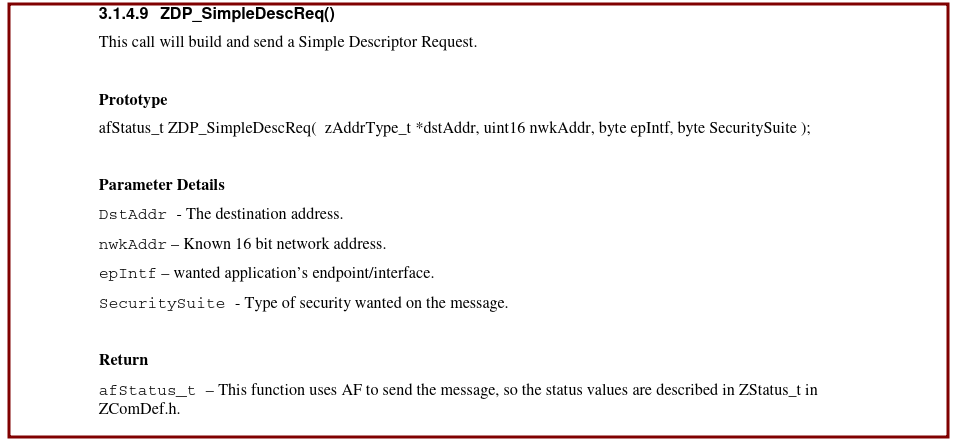
\includegraphics[width=1\textwidth]{media/z-stack-api-excerpt.png}
  \caption{Z-Stack API Auszug}
\end{figure}

In diesem Beispiel wird beschrieben, wie man einen SimpleDescriptor-Request an ein Zigbee-Device versendet. Dieser Aufruf ist entsprechend Parametrierbar,
und wird zur Abfrage der verfügbaren Endpunkte eines Gerätes nach dessen Beitritt in das Netzwerk abgefragt.

\subsubsection{zigbee-herdman-converters}

Dieser Konverter kann proprietäre Cluster die durch Geräte exposed werden umwandeln in Standard Cluster. Mit diesem Converter lassen sich proprietäre Cluster von Geräte
so adaptieren, dass sie nach Wunsch gesteuert und ausgelesen werden können.

\subsubsection{zigbee2mqtt}

Das Hauptmodul stellt die WebGui sowie eine Webanwendung mit einer SQLite Datenbank. Die Webanwendung und die Datenbank
verwalten den Zustand des Netzwerkes und die angebundenen Geräte. Die WebGUI dient zur Administration des Koordinators. 

\begin{figure}[H]
  \centering
  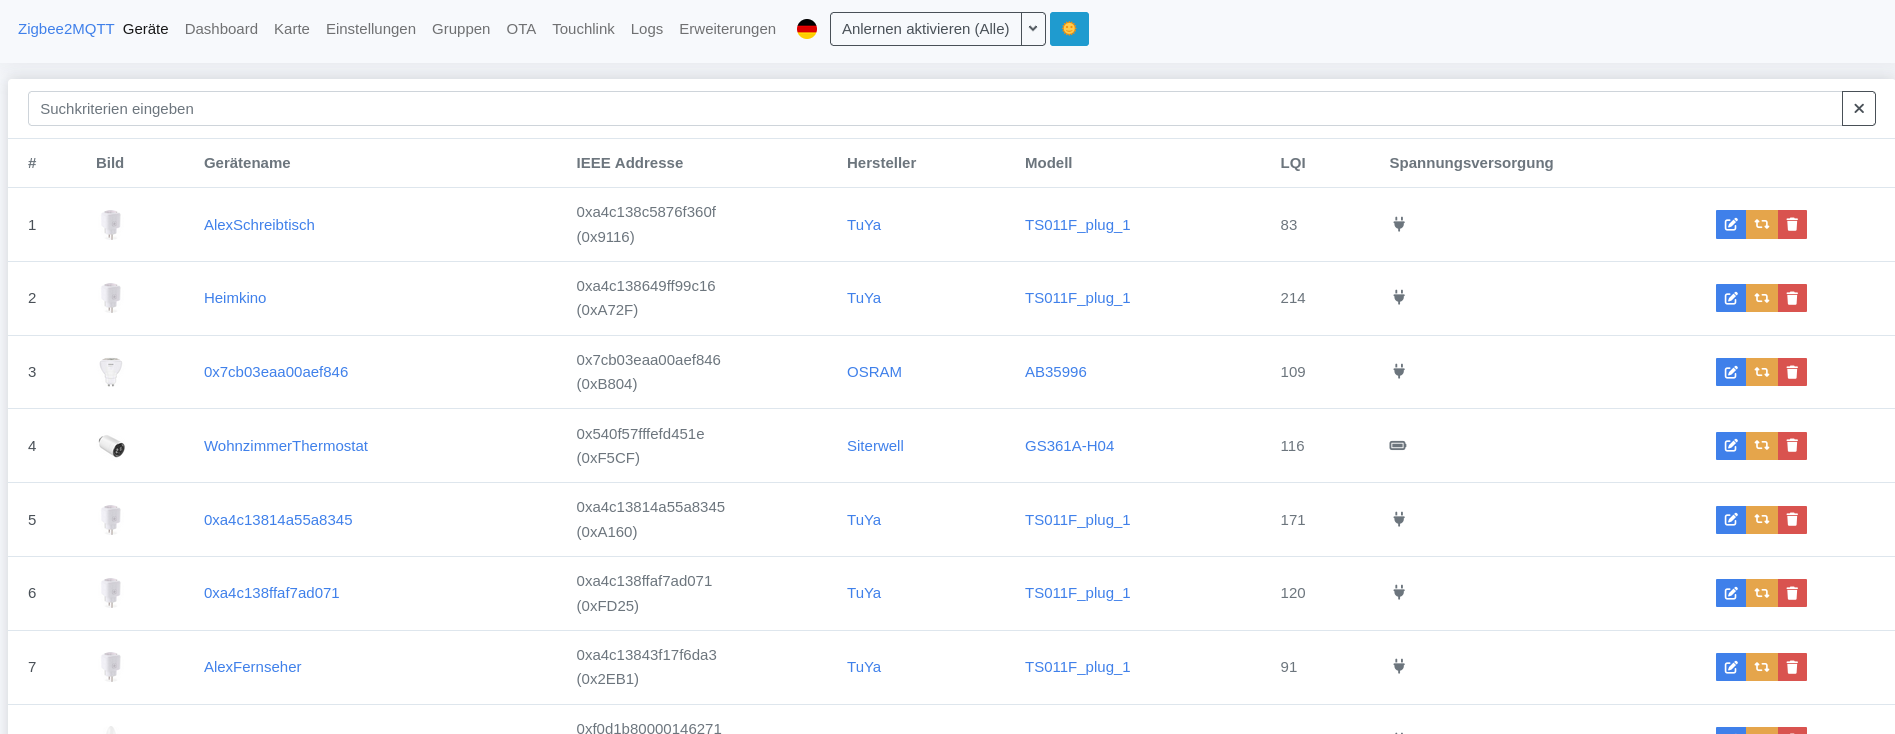
\includegraphics[width=1\textwidth]{media/z2m.png}
  \caption{zigbee2mqtt Webfrontend}
\end{figure}

Die WebGUI enthält eine große Anzahl von Funktionen, die weitaus tiefer reichen als für die Nutzung notwendig sind.
Prinzipiell sind die meißten ZigBee Geräte Kompatibel, wenn ein Community Mitglied dieses bereits in der Anwendung
angelegt hat. Es ist auch möglich, eigene Beschreibungen für nich nicht unterstützte Geräte zu erstellen.\\

\begin{figure}[H]
  \centering
  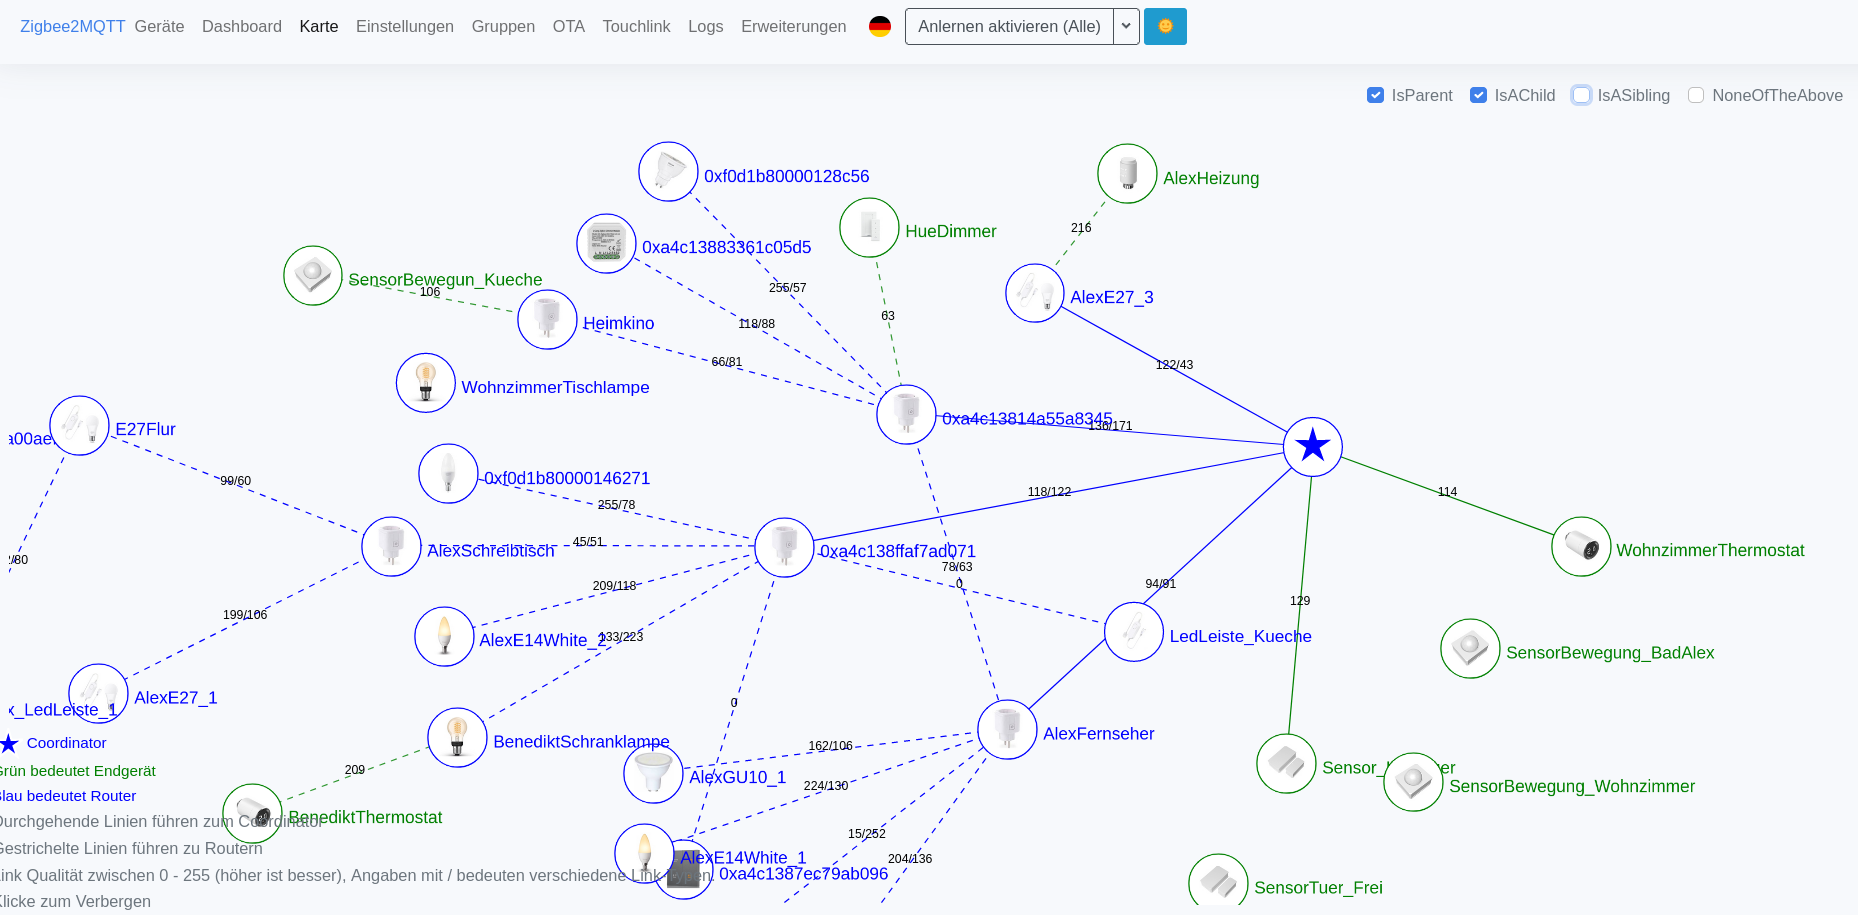
\includegraphics[width=1\textwidth]{media/z2m-map.png}
  \caption{zigbee2mqtt Netzwerkvisualisierung}
\end{figure}

Das Netzwerk lässt sich in einer dynamischen Übersicht visualisieren. Hier die aktiv genutzen Verbindung zwischen den Geräten. 

\subsection{Wireshark}

Wireshark ist eine quelloffene Anwendung um Datenstöme Mitzuschneiden und zu Untersuchen. Es kann durch Verwendung
von Packetsniffern wie nPcap verschiedenste Medien wie zum Beispiel Ethernet und USB mit entsprechenden Protokollen
verarbeiten.

\todo{Screenshot Wireshark mit Zigbee Paketen}

\subsection{zbWireshark}

Dies ist ein Script aus einem Git-Hub Repository. Mit diesem Script lässt sich Wireshark starten und anschließend Pakete über den 
ZigBee Sniffer Stick mitschreiben.

\url{https://github.com/silicrax/killerbee/tree/master/tools}

\subsection{Ansible}

Ansible ist ein Tool zur IT-Automatisierung. Arbeitsabläufe lassen sich ebenfall gut strukturiert in YAML definieren. Ansible verbindet sich per SSH 
mit den zu konfigurierenden Hosts und führt Python Module aus. Hosts lassen sich in Gruppen, und Tasks in sogenannten Rollen sammeln. So ist es möglich,
eine Gruppe von Hosts die Rolle \grqq Webapplikation \grqq{}, und einer Gruppe von anderen Hosts der Gruppe \grqq Datenbank \grqq{} zuweisen. 
Eine Zuweisung von Rollen sihet folgendermaßen aus:
\begin{lstlisting}
  - name: Deploy the Lab
  hosts: localhost
  roles:
    - DeployDocker
    - DeployLabUtils
\end{lstlisting}

In diesem Beispiel wird auf dem lokalen Host Docker installiert, und das ZigBee Praktikum vorbereitet.

\subsection{}
